\hypertarget{a00014}{
\section{Dokumentacja klasy ASS8.Klient.Konfiguracja}
\label{d2/de7/a00014}\index{ASS8::Klient::Konfiguracja@{ASS8::Klient::Konfiguracja}}
}
Klasa wyświetlająca okno do zmiany konfiguracji.  


Diagram współpracy dla ASS8.Klient.Konfiguracja:\nopagebreak
\begin{figure}[H]
\begin{center}
\leavevmode
\includegraphics[width=226pt]{d1/db7/a00157}
\end{center}
\end{figure}
\subsection*{Metody publiczne}
\begin{CompactItemize}
\item 
\hyperlink{a00014_b298e3bc6d95ff4bb409a69a84598ea6}{Konfiguracja} (Form log, \hyperlink{a00013}{komunikacja} kom)
\begin{CompactList}\small\item\em Konstruktor klasy, inicjalizuje wszystkie pola w formularzu. \item\end{CompactList}\end{CompactItemize}
\subsection*{Atrybuty publiczne}
\begin{CompactItemize}
\item 
int \hyperlink{a00014_b484254239ce03aa12ad870b9c5454fb}{sekundy}
\end{CompactItemize}
\subsection*{Właściwości}
\begin{CompactItemize}
\item 
\hyperlink{a00013}{komunikacja} \hyperlink{a00014_ebc21fd88f797ade28feaaa274769fa8}{KomClass}\hspace{0.3cm}{\tt  \mbox{[}get, set\mbox{]}}
\end{CompactItemize}
\subsection*{Metody prywatne}
\begin{CompactItemize}
\item 
void \hyperlink{a00014_49a6172f91f2b718c2838960918afba7}{automatyczneSpr} (object o)
\begin{CompactList}\small\item\em Wysyołuje automatyczne sprawdzanie katalogu co określona ilość czasu. \item\end{CompactList}\item 
void \hyperlink{a00014_43e125d87ba2497d29d9ad6ea456c62d}{btnSciezka\_\-Click} (object sender, EventArgs e)
\begin{CompactList}\small\item\em Wyświetla okno do wyboru nowego folderu. \item\end{CompactList}\item 
void \hyperlink{a00014_f679b61007ce606b466155103b678d40}{ASS8\_\-\_\-\_\-Konfiguracja\_\-FormClosing} (object sender, FormClosingEventArgs e)
\begin{CompactList}\small\item\em Obsługa zamykania formularza. \item\end{CompactList}\item 
void \hyperlink{a00014_321774e21dbe196e41840825cbe7c915}{tcmsKonfiguracja\_\-Click} (object sender, EventArgs e)
\begin{CompactList}\small\item\em Obsługa opcji w trayu wyświetlającej okno konfiguracji. \item\end{CompactList}\item 
void \hyperlink{a00014_e273925aef74f02490b3a4ac6af6b779}{tcmsZnajomi\_\-Click} (object sender, EventArgs e)
\begin{CompactList}\small\item\em Obsługa opcji w trayu wyświetlającej okno znajomych. \item\end{CompactList}\item 
void \hyperlink{a00014_320235785478082ecc1aa03461bf2784}{cmsWyloguj\_\-Click} (object sender, EventArgs e)
\begin{CompactList}\small\item\em Obsługa opcji w trayu wylogowującej użytkownika. \item\end{CompactList}\item 
void \hyperlink{a00014_2f9d0525ac9851488072e040aaf7651c}{tcmsZakoncz\_\-Click} (object sender, EventArgs e)
\begin{CompactList}\small\item\em Obsługa opcji w trayu zamykającej aplikację. \item\end{CompactList}\item 
void \hyperlink{a00014_91afe239346bf7e48bbe5472a7c77dee}{tcmsStop\_\-Click} (object sender, EventArgs e)
\begin{CompactList}\small\item\em Obsługa opcji w trayu stopującej automatyczną aktualizację. \item\end{CompactList}\item 
void \hyperlink{a00014_6b5fcbc389c958d850ae624c7c202372}{tcmsStart\_\-Click} (object sender, EventArgs e)
\begin{CompactList}\small\item\em Obsługa opcji w trayu startującą automatyczną aktualizację. \item\end{CompactList}\item 
void \hyperlink{a00014_c585e179ba2eae275bc72800350139ed}{label4\_\-Click} (object sender, EventArgs e)
\item 
void \hyperlink{a00014_9fae1354592491cc868938a644d08225}{checkBox1\_\-CheckedChanged} (object sender, EventArgs e)
\begin{CompactList}\small\item\em Funkcja wywoływana podczas zmiany checkboxa i wywołująca odpowiednie zmiany. \item\end{CompactList}\item 
void \hyperlink{a00014_4d234b74e7e673575fb90c7b41cdd79c}{chbUwierzytelnienie\_\-CheckedChanged} (object sender, EventArgs e)
\begin{CompactList}\small\item\em Funkcja wywoływana podczas zmiany checkboxa i wywołująca odpowiednie zmiany. \item\end{CompactList}\item 
void \hyperlink{a00014_12f013346e6d02fe69877467ca551ef3}{btnZapisz\_\-Click} (object sender, EventArgs e)
\begin{CompactList}\small\item\em Obsluga przycisku zapisującego \hyperlink{a00028}{ustawienia}. Ustawienia są zapisywane do pliku. \item\end{CompactList}\item 
void \hyperlink{a00014_9d2b40a270afe4ddbcc6059e2e6d940b}{zmianaFolderu} (object o)
\begin{CompactList}\small\item\em Funkcja odpowiedzialna za zmiane folderu aktualizacji. \item\end{CompactList}\item 
void \hyperlink{a00014_f95affc14a6ee755996b87db35881a75}{btnAnuluj\_\-Click} (object sender, EventArgs e)
\begin{CompactList}\small\item\em Obsługa przycisku Zamknij. \item\end{CompactList}\end{CompactItemize}
\subsection*{Atrybuty prywatne}
\begin{CompactItemize}
\item 
XmlSerializerNamespaces \hyperlink{a00014_a9ee3b6dc3dc3b9960e784cd32f1cf60}{names}
\item 
\hyperlink{a00013}{komunikacja} \hyperlink{a00014_092fa470ee5f9059cdfda4533edff021}{k}
\item 
bool \hyperlink{a00014_38ea713cadc6819701e3313479fbd000}{close} = false
\item 
Form \hyperlink{a00014_59cabf8f3e48082c0ffa5f7da06fc270}{loginForm}
\item 
\hyperlink{a00037}{zarzadca} \hyperlink{a00014_4a874d85030babce8df85e2dadf9577e}{z}
\item 
int \hyperlink{a00014_3817bb57be51df140314a2da2aa5ba7e}{bledyKontrola}
\item 
string \hyperlink{a00014_e7c5ada1eda848babdd60e4e8c79b819}{fol}
\end{CompactItemize}


\subsection{Opis szczegółowy}
Klasa wyświetlająca okno do zmiany konfiguracji. 



Definicja w linii 19 pliku ASS8 - Konfiguracja.cs.

\subsection{Dokumentacja konstruktora i destruktora}
\hypertarget{a00014_b298e3bc6d95ff4bb409a69a84598ea6}{
\index{ASS8::Klient::Konfiguracja@{ASS8::Klient::Konfiguracja}!Konfiguracja@{Konfiguracja}}
\index{Konfiguracja@{Konfiguracja}!ASS8::Klient::Konfiguracja@{ASS8::Klient::Konfiguracja}}
\subsubsection[{Konfiguracja}]{\setlength{\rightskip}{0pt plus 5cm}ASS8.Klient.Konfiguracja.Konfiguracja (Form {\em log}, \/  {\bf komunikacja} {\em kom})}}
\label{d2/de7/a00014_b298e3bc6d95ff4bb409a69a84598ea6}


Konstruktor klasy, inicjalizuje wszystkie pola w formularzu. 

\begin{Desc}
\item[Parametry:]
\begin{description}
\item[{\em log}]Formularz logowania\item[{\em kom}]Zmienna do komunikacji sieciowej\end{description}
\end{Desc}


Definicja w linii 59 pliku ASS8 - Konfiguracja.cs.

\subsection{Dokumentacja funkcji składowych}
\hypertarget{a00014_f679b61007ce606b466155103b678d40}{
\index{ASS8::Klient::Konfiguracja@{ASS8::Klient::Konfiguracja}!ASS8\_\-\_\-\_\-Konfiguracja\_\-FormClosing@{ASS8\_\-\_\-\_\-Konfiguracja\_\-FormClosing}}
\index{ASS8\_\-\_\-\_\-Konfiguracja\_\-FormClosing@{ASS8\_\-\_\-\_\-Konfiguracja\_\-FormClosing}!ASS8::Klient::Konfiguracja@{ASS8::Klient::Konfiguracja}}
\subsubsection[{ASS8\_\-\_\-\_\-Konfiguracja\_\-FormClosing}]{\setlength{\rightskip}{0pt plus 5cm}void ASS8.Klient.Konfiguracja.ASS8\_\-\_\-\_\-Konfiguracja\_\-FormClosing (object {\em sender}, \/  FormClosingEventArgs {\em e})\hspace{0.3cm}{\tt  \mbox{[}private\mbox{]}}}}
\label{d2/de7/a00014_f679b61007ce606b466155103b678d40}


Obsługa zamykania formularza. 

\begin{Desc}
\item[Parametry:]
\begin{description}
\item[{\em sender}]\item[{\em e}]\end{description}
\end{Desc}


Definicja w linii 156 pliku ASS8 - Konfiguracja.cs.\hypertarget{a00014_49a6172f91f2b718c2838960918afba7}{
\index{ASS8::Klient::Konfiguracja@{ASS8::Klient::Konfiguracja}!automatyczneSpr@{automatyczneSpr}}
\index{automatyczneSpr@{automatyczneSpr}!ASS8::Klient::Konfiguracja@{ASS8::Klient::Konfiguracja}}
\subsubsection[{automatyczneSpr}]{\setlength{\rightskip}{0pt plus 5cm}void ASS8.Klient.Konfiguracja.automatyczneSpr (object {\em o})\hspace{0.3cm}{\tt  \mbox{[}private\mbox{]}}}}
\label{d2/de7/a00014_49a6172f91f2b718c2838960918afba7}


Wysyołuje automatyczne sprawdzanie katalogu co określona ilość czasu. 

\begin{Desc}
\item[Parametry:]
\begin{description}
\item[{\em o}]Lista zmienny niezbędnych do utworzenia połączenia (utworzenia klasy \hyperlink{a00013}{komunikacja})\end{description}
\end{Desc}


Definicja w linii 33 pliku ASS8 - Konfiguracja.cs.

Oto graf wywołań dla tej funkcji:\nopagebreak
\begin{figure}[H]
\begin{center}
\leavevmode
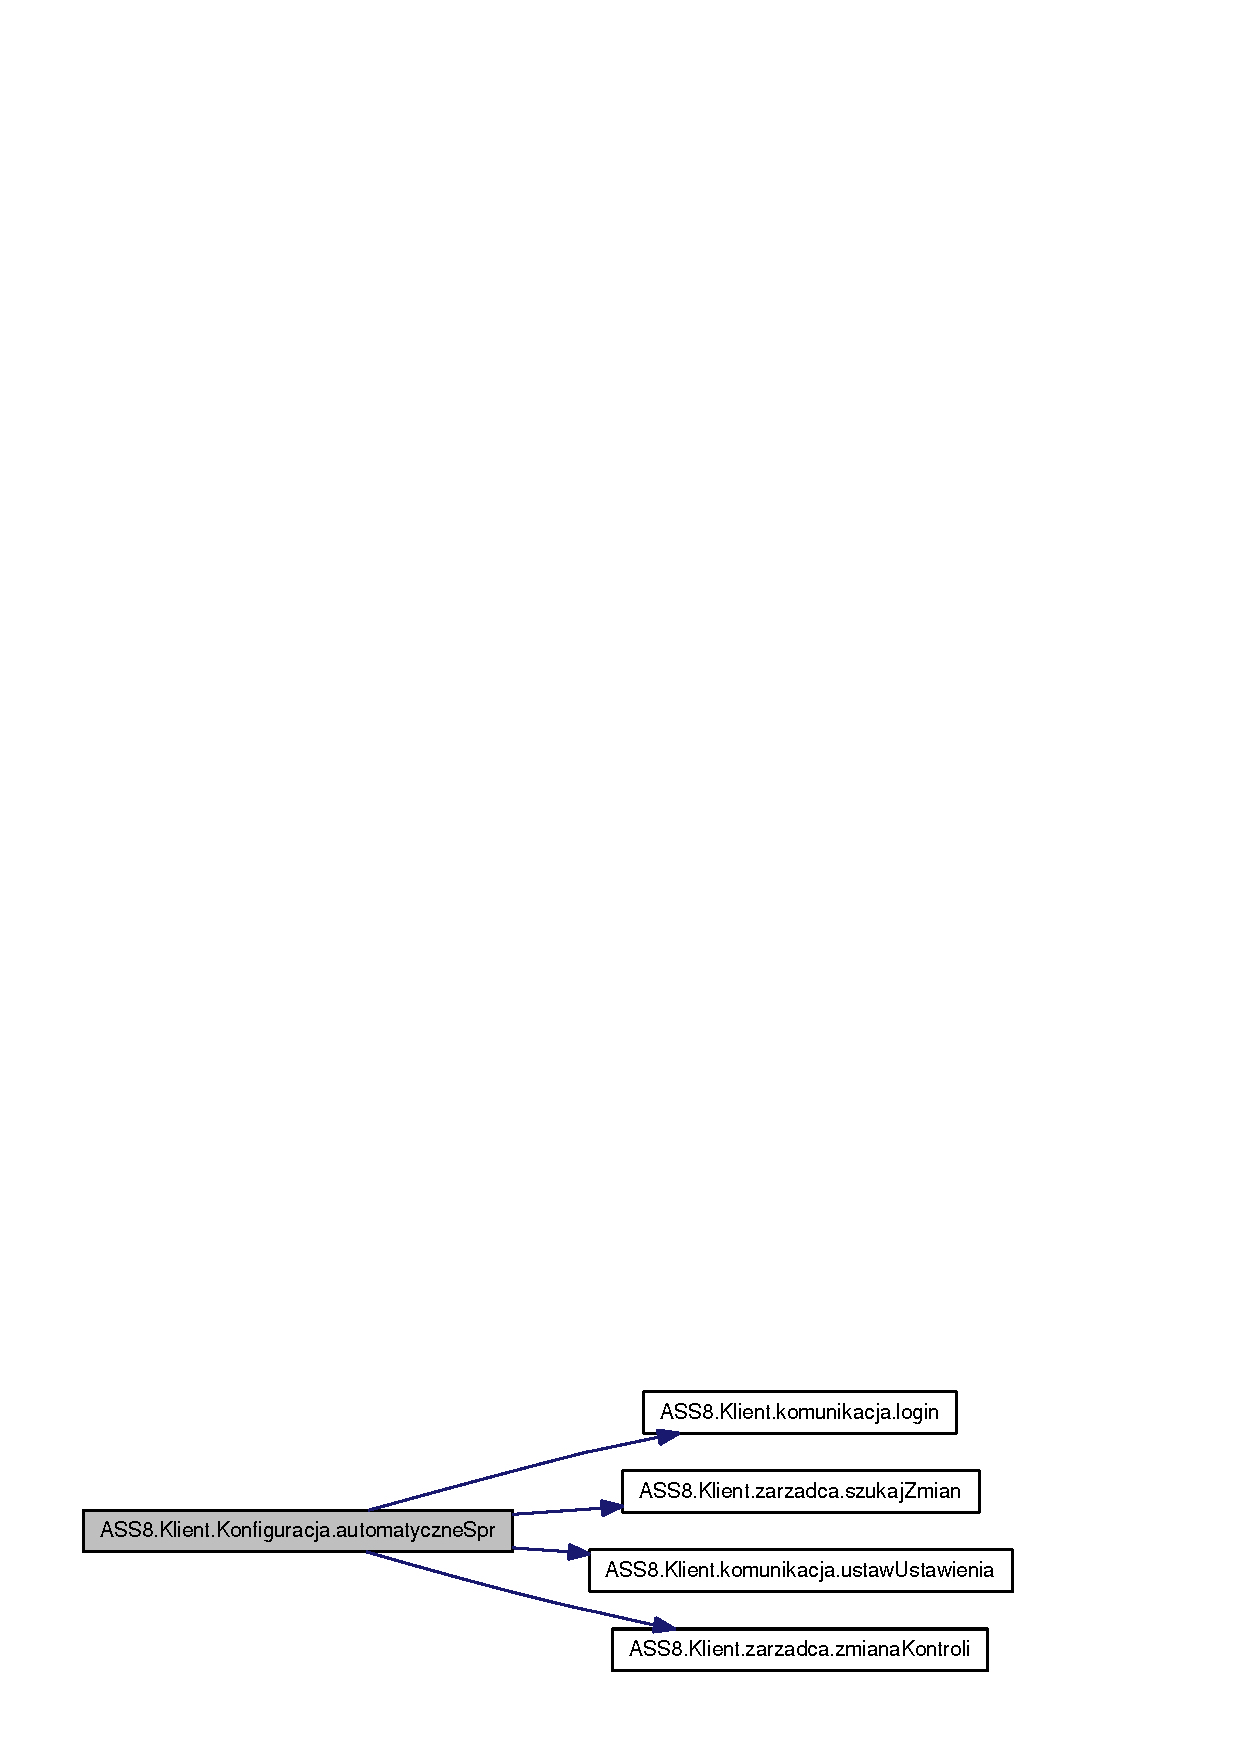
\includegraphics[width=245pt]{d2/de7/a00014_49a6172f91f2b718c2838960918afba7_cgraph}
\end{center}
\end{figure}
\hypertarget{a00014_f95affc14a6ee755996b87db35881a75}{
\index{ASS8::Klient::Konfiguracja@{ASS8::Klient::Konfiguracja}!btnAnuluj\_\-Click@{btnAnuluj\_\-Click}}
\index{btnAnuluj\_\-Click@{btnAnuluj\_\-Click}!ASS8::Klient::Konfiguracja@{ASS8::Klient::Konfiguracja}}
\subsubsection[{btnAnuluj\_\-Click}]{\setlength{\rightskip}{0pt plus 5cm}void ASS8.Klient.Konfiguracja.btnAnuluj\_\-Click (object {\em sender}, \/  EventArgs {\em e})\hspace{0.3cm}{\tt  \mbox{[}private\mbox{]}}}}
\label{d2/de7/a00014_f95affc14a6ee755996b87db35881a75}


Obsługa przycisku Zamknij. 

\begin{Desc}
\item[Parametry:]
\begin{description}
\item[{\em sender}]\item[{\em e}]\end{description}
\end{Desc}


Definicja w linii 339 pliku ASS8 - Konfiguracja.cs.\hypertarget{a00014_43e125d87ba2497d29d9ad6ea456c62d}{
\index{ASS8::Klient::Konfiguracja@{ASS8::Klient::Konfiguracja}!btnSciezka\_\-Click@{btnSciezka\_\-Click}}
\index{btnSciezka\_\-Click@{btnSciezka\_\-Click}!ASS8::Klient::Konfiguracja@{ASS8::Klient::Konfiguracja}}
\subsubsection[{btnSciezka\_\-Click}]{\setlength{\rightskip}{0pt plus 5cm}void ASS8.Klient.Konfiguracja.btnSciezka\_\-Click (object {\em sender}, \/  EventArgs {\em e})\hspace{0.3cm}{\tt  \mbox{[}private\mbox{]}}}}
\label{d2/de7/a00014_43e125d87ba2497d29d9ad6ea456c62d}


Wyświetla okno do wyboru nowego folderu. 

\begin{Desc}
\item[Parametry:]
\begin{description}
\item[{\em sender}]\item[{\em e}]\end{description}
\end{Desc}


Definicja w linii 143 pliku ASS8 - Konfiguracja.cs.\hypertarget{a00014_12f013346e6d02fe69877467ca551ef3}{
\index{ASS8::Klient::Konfiguracja@{ASS8::Klient::Konfiguracja}!btnZapisz\_\-Click@{btnZapisz\_\-Click}}
\index{btnZapisz\_\-Click@{btnZapisz\_\-Click}!ASS8::Klient::Konfiguracja@{ASS8::Klient::Konfiguracja}}
\subsubsection[{btnZapisz\_\-Click}]{\setlength{\rightskip}{0pt plus 5cm}void ASS8.Klient.Konfiguracja.btnZapisz\_\-Click (object {\em sender}, \/  EventArgs {\em e})\hspace{0.3cm}{\tt  \mbox{[}private\mbox{]}}}}
\label{d2/de7/a00014_12f013346e6d02fe69877467ca551ef3}


Obsluga przycisku zapisującego \hyperlink{a00028}{ustawienia}. Ustawienia są zapisywane do pliku. 

\begin{Desc}
\item[Parametry:]
\begin{description}
\item[{\em sender}]\item[{\em e}]\end{description}
\end{Desc}


Definicja w linii 263 pliku ASS8 - Konfiguracja.cs.\hypertarget{a00014_4d234b74e7e673575fb90c7b41cdd79c}{
\index{ASS8::Klient::Konfiguracja@{ASS8::Klient::Konfiguracja}!chbUwierzytelnienie\_\-CheckedChanged@{chbUwierzytelnienie\_\-CheckedChanged}}
\index{chbUwierzytelnienie\_\-CheckedChanged@{chbUwierzytelnienie\_\-CheckedChanged}!ASS8::Klient::Konfiguracja@{ASS8::Klient::Konfiguracja}}
\subsubsection[{chbUwierzytelnienie\_\-CheckedChanged}]{\setlength{\rightskip}{0pt plus 5cm}void ASS8.Klient.Konfiguracja.chbUwierzytelnienie\_\-CheckedChanged (object {\em sender}, \/  EventArgs {\em e})\hspace{0.3cm}{\tt  \mbox{[}private\mbox{]}}}}
\label{d2/de7/a00014_4d234b74e7e673575fb90c7b41cdd79c}


Funkcja wywoływana podczas zmiany checkboxa i wywołująca odpowiednie zmiany. 

\begin{Desc}
\item[Parametry:]
\begin{description}
\item[{\em sender}]\item[{\em e}]\end{description}
\end{Desc}


Definicja w linii 251 pliku ASS8 - Konfiguracja.cs.\hypertarget{a00014_9fae1354592491cc868938a644d08225}{
\index{ASS8::Klient::Konfiguracja@{ASS8::Klient::Konfiguracja}!checkBox1\_\-CheckedChanged@{checkBox1\_\-CheckedChanged}}
\index{checkBox1\_\-CheckedChanged@{checkBox1\_\-CheckedChanged}!ASS8::Klient::Konfiguracja@{ASS8::Klient::Konfiguracja}}
\subsubsection[{checkBox1\_\-CheckedChanged}]{\setlength{\rightskip}{0pt plus 5cm}void ASS8.Klient.Konfiguracja.checkBox1\_\-CheckedChanged (object {\em sender}, \/  EventArgs {\em e})\hspace{0.3cm}{\tt  \mbox{[}private\mbox{]}}}}
\label{d2/de7/a00014_9fae1354592491cc868938a644d08225}


Funkcja wywoływana podczas zmiany checkboxa i wywołująca odpowiednie zmiany. 

\begin{Desc}
\item[Parametry:]
\begin{description}
\item[{\em sender}]\item[{\em e}]\end{description}
\end{Desc}


Definicja w linii 237 pliku ASS8 - Konfiguracja.cs.\hypertarget{a00014_320235785478082ecc1aa03461bf2784}{
\index{ASS8::Klient::Konfiguracja@{ASS8::Klient::Konfiguracja}!cmsWyloguj\_\-Click@{cmsWyloguj\_\-Click}}
\index{cmsWyloguj\_\-Click@{cmsWyloguj\_\-Click}!ASS8::Klient::Konfiguracja@{ASS8::Klient::Konfiguracja}}
\subsubsection[{cmsWyloguj\_\-Click}]{\setlength{\rightskip}{0pt plus 5cm}void ASS8.Klient.Konfiguracja.cmsWyloguj\_\-Click (object {\em sender}, \/  EventArgs {\em e})\hspace{0.3cm}{\tt  \mbox{[}private\mbox{]}}}}
\label{d2/de7/a00014_320235785478082ecc1aa03461bf2784}


Obsługa opcji w trayu wylogowującej użytkownika. 

\begin{Desc}
\item[Parametry:]
\begin{description}
\item[{\em sender}]\item[{\em e}]\end{description}
\end{Desc}


Definicja w linii 189 pliku ASS8 - Konfiguracja.cs.\hypertarget{a00014_c585e179ba2eae275bc72800350139ed}{
\index{ASS8::Klient::Konfiguracja@{ASS8::Klient::Konfiguracja}!label4\_\-Click@{label4\_\-Click}}
\index{label4\_\-Click@{label4\_\-Click}!ASS8::Klient::Konfiguracja@{ASS8::Klient::Konfiguracja}}
\subsubsection[{label4\_\-Click}]{\setlength{\rightskip}{0pt plus 5cm}void ASS8.Klient.Konfiguracja.label4\_\-Click (object {\em sender}, \/  EventArgs {\em e})\hspace{0.3cm}{\tt  \mbox{[}private\mbox{]}}}}
\label{d2/de7/a00014_c585e179ba2eae275bc72800350139ed}




Definicja w linii 228 pliku ASS8 - Konfiguracja.cs.\hypertarget{a00014_321774e21dbe196e41840825cbe7c915}{
\index{ASS8::Klient::Konfiguracja@{ASS8::Klient::Konfiguracja}!tcmsKonfiguracja\_\-Click@{tcmsKonfiguracja\_\-Click}}
\index{tcmsKonfiguracja\_\-Click@{tcmsKonfiguracja\_\-Click}!ASS8::Klient::Konfiguracja@{ASS8::Klient::Konfiguracja}}
\subsubsection[{tcmsKonfiguracja\_\-Click}]{\setlength{\rightskip}{0pt plus 5cm}void ASS8.Klient.Konfiguracja.tcmsKonfiguracja\_\-Click (object {\em sender}, \/  EventArgs {\em e})\hspace{0.3cm}{\tt  \mbox{[}private\mbox{]}}}}
\label{d2/de7/a00014_321774e21dbe196e41840825cbe7c915}


Obsługa opcji w trayu wyświetlającej okno konfiguracji. 

\begin{Desc}
\item[Parametry:]
\begin{description}
\item[{\em sender}]\item[{\em e}]\end{description}
\end{Desc}


Definicja w linii 169 pliku ASS8 - Konfiguracja.cs.\hypertarget{a00014_6b5fcbc389c958d850ae624c7c202372}{
\index{ASS8::Klient::Konfiguracja@{ASS8::Klient::Konfiguracja}!tcmsStart\_\-Click@{tcmsStart\_\-Click}}
\index{tcmsStart\_\-Click@{tcmsStart\_\-Click}!ASS8::Klient::Konfiguracja@{ASS8::Klient::Konfiguracja}}
\subsubsection[{tcmsStart\_\-Click}]{\setlength{\rightskip}{0pt plus 5cm}void ASS8.Klient.Konfiguracja.tcmsStart\_\-Click (object {\em sender}, \/  EventArgs {\em e})\hspace{0.3cm}{\tt  \mbox{[}private\mbox{]}}}}
\label{d2/de7/a00014_6b5fcbc389c958d850ae624c7c202372}


Obsługa opcji w trayu startującą automatyczną aktualizację. 

\begin{Desc}
\item[Parametry:]
\begin{description}
\item[{\em sender}]\item[{\em e}]\end{description}
\end{Desc}


Definicja w linii 221 pliku ASS8 - Konfiguracja.cs.\hypertarget{a00014_91afe239346bf7e48bbe5472a7c77dee}{
\index{ASS8::Klient::Konfiguracja@{ASS8::Klient::Konfiguracja}!tcmsStop\_\-Click@{tcmsStop\_\-Click}}
\index{tcmsStop\_\-Click@{tcmsStop\_\-Click}!ASS8::Klient::Konfiguracja@{ASS8::Klient::Konfiguracja}}
\subsubsection[{tcmsStop\_\-Click}]{\setlength{\rightskip}{0pt plus 5cm}void ASS8.Klient.Konfiguracja.tcmsStop\_\-Click (object {\em sender}, \/  EventArgs {\em e})\hspace{0.3cm}{\tt  \mbox{[}private\mbox{]}}}}
\label{d2/de7/a00014_91afe239346bf7e48bbe5472a7c77dee}


Obsługa opcji w trayu stopującej automatyczną aktualizację. 

\begin{Desc}
\item[Parametry:]
\begin{description}
\item[{\em sender}]\item[{\em e}]\end{description}
\end{Desc}


Definicja w linii 210 pliku ASS8 - Konfiguracja.cs.\hypertarget{a00014_2f9d0525ac9851488072e040aaf7651c}{
\index{ASS8::Klient::Konfiguracja@{ASS8::Klient::Konfiguracja}!tcmsZakoncz\_\-Click@{tcmsZakoncz\_\-Click}}
\index{tcmsZakoncz\_\-Click@{tcmsZakoncz\_\-Click}!ASS8::Klient::Konfiguracja@{ASS8::Klient::Konfiguracja}}
\subsubsection[{tcmsZakoncz\_\-Click}]{\setlength{\rightskip}{0pt plus 5cm}void ASS8.Klient.Konfiguracja.tcmsZakoncz\_\-Click (object {\em sender}, \/  EventArgs {\em e})\hspace{0.3cm}{\tt  \mbox{[}private\mbox{]}}}}
\label{d2/de7/a00014_2f9d0525ac9851488072e040aaf7651c}


Obsługa opcji w trayu zamykającej aplikację. 

\begin{Desc}
\item[Parametry:]
\begin{description}
\item[{\em sender}]\item[{\em e}]\end{description}
\end{Desc}


Definicja w linii 201 pliku ASS8 - Konfiguracja.cs.\hypertarget{a00014_e273925aef74f02490b3a4ac6af6b779}{
\index{ASS8::Klient::Konfiguracja@{ASS8::Klient::Konfiguracja}!tcmsZnajomi\_\-Click@{tcmsZnajomi\_\-Click}}
\index{tcmsZnajomi\_\-Click@{tcmsZnajomi\_\-Click}!ASS8::Klient::Konfiguracja@{ASS8::Klient::Konfiguracja}}
\subsubsection[{tcmsZnajomi\_\-Click}]{\setlength{\rightskip}{0pt plus 5cm}void ASS8.Klient.Konfiguracja.tcmsZnajomi\_\-Click (object {\em sender}, \/  EventArgs {\em e})\hspace{0.3cm}{\tt  \mbox{[}private\mbox{]}}}}
\label{d2/de7/a00014_e273925aef74f02490b3a4ac6af6b779}


Obsługa opcji w trayu wyświetlającej okno znajomych. 

\begin{Desc}
\item[Parametry:]
\begin{description}
\item[{\em sender}]\item[{\em e}]\end{description}
\end{Desc}


Definicja w linii 178 pliku ASS8 - Konfiguracja.cs.\hypertarget{a00014_9d2b40a270afe4ddbcc6059e2e6d940b}{
\index{ASS8::Klient::Konfiguracja@{ASS8::Klient::Konfiguracja}!zmianaFolderu@{zmianaFolderu}}
\index{zmianaFolderu@{zmianaFolderu}!ASS8::Klient::Konfiguracja@{ASS8::Klient::Konfiguracja}}
\subsubsection[{zmianaFolderu}]{\setlength{\rightskip}{0pt plus 5cm}void ASS8.Klient.Konfiguracja.zmianaFolderu (object {\em o})\hspace{0.3cm}{\tt  \mbox{[}private\mbox{]}}}}
\label{d2/de7/a00014_9d2b40a270afe4ddbcc6059e2e6d940b}


Funkcja odpowiedzialna za zmiane folderu aktualizacji. 

\begin{Desc}
\item[Parametry:]
\begin{description}
\item[{\em o}]\end{description}
\end{Desc}


Definicja w linii 327 pliku ASS8 - Konfiguracja.cs.

\subsection{Dokumentacja atrybutów składowych}
\hypertarget{a00014_3817bb57be51df140314a2da2aa5ba7e}{
\index{ASS8::Klient::Konfiguracja@{ASS8::Klient::Konfiguracja}!bledyKontrola@{bledyKontrola}}
\index{bledyKontrola@{bledyKontrola}!ASS8::Klient::Konfiguracja@{ASS8::Klient::Konfiguracja}}
\subsubsection[{bledyKontrola}]{\setlength{\rightskip}{0pt plus 5cm}int {\bf ASS8.Klient.Konfiguracja.bledyKontrola}\hspace{0.3cm}{\tt  \mbox{[}private\mbox{]}}}}
\label{d2/de7/a00014_3817bb57be51df140314a2da2aa5ba7e}




Definicja w linii 27 pliku ASS8 - Konfiguracja.cs.\hypertarget{a00014_38ea713cadc6819701e3313479fbd000}{
\index{ASS8::Klient::Konfiguracja@{ASS8::Klient::Konfiguracja}!close@{close}}
\index{close@{close}!ASS8::Klient::Konfiguracja@{ASS8::Klient::Konfiguracja}}
\subsubsection[{close}]{\setlength{\rightskip}{0pt plus 5cm}bool {\bf ASS8.Klient.Konfiguracja.close} = false\hspace{0.3cm}{\tt  \mbox{[}private\mbox{]}}}}
\label{d2/de7/a00014_38ea713cadc6819701e3313479fbd000}




Definicja w linii 23 pliku ASS8 - Konfiguracja.cs.\hypertarget{a00014_e7c5ada1eda848babdd60e4e8c79b819}{
\index{ASS8::Klient::Konfiguracja@{ASS8::Klient::Konfiguracja}!fol@{fol}}
\index{fol@{fol}!ASS8::Klient::Konfiguracja@{ASS8::Klient::Konfiguracja}}
\subsubsection[{fol}]{\setlength{\rightskip}{0pt plus 5cm}string {\bf ASS8.Klient.Konfiguracja.fol}\hspace{0.3cm}{\tt  \mbox{[}private\mbox{]}}}}
\label{d2/de7/a00014_e7c5ada1eda848babdd60e4e8c79b819}




Definicja w linii 28 pliku ASS8 - Konfiguracja.cs.\hypertarget{a00014_092fa470ee5f9059cdfda4533edff021}{
\index{ASS8::Klient::Konfiguracja@{ASS8::Klient::Konfiguracja}!k@{k}}
\index{k@{k}!ASS8::Klient::Konfiguracja@{ASS8::Klient::Konfiguracja}}
\subsubsection[{k}]{\setlength{\rightskip}{0pt plus 5cm}{\bf komunikacja} {\bf ASS8.Klient.Konfiguracja.k}\hspace{0.3cm}{\tt  \mbox{[}private\mbox{]}}}}
\label{d2/de7/a00014_092fa470ee5f9059cdfda4533edff021}




Definicja w linii 22 pliku ASS8 - Konfiguracja.cs.\hypertarget{a00014_59cabf8f3e48082c0ffa5f7da06fc270}{
\index{ASS8::Klient::Konfiguracja@{ASS8::Klient::Konfiguracja}!loginForm@{loginForm}}
\index{loginForm@{loginForm}!ASS8::Klient::Konfiguracja@{ASS8::Klient::Konfiguracja}}
\subsubsection[{loginForm}]{\setlength{\rightskip}{0pt plus 5cm}Form {\bf ASS8.Klient.Konfiguracja.loginForm}\hspace{0.3cm}{\tt  \mbox{[}private\mbox{]}}}}
\label{d2/de7/a00014_59cabf8f3e48082c0ffa5f7da06fc270}




Definicja w linii 24 pliku ASS8 - Konfiguracja.cs.\hypertarget{a00014_a9ee3b6dc3dc3b9960e784cd32f1cf60}{
\index{ASS8::Klient::Konfiguracja@{ASS8::Klient::Konfiguracja}!names@{names}}
\index{names@{names}!ASS8::Klient::Konfiguracja@{ASS8::Klient::Konfiguracja}}
\subsubsection[{names}]{\setlength{\rightskip}{0pt plus 5cm}XmlSerializerNamespaces {\bf ASS8.Klient.Konfiguracja.names}\hspace{0.3cm}{\tt  \mbox{[}private\mbox{]}}}}
\label{d2/de7/a00014_a9ee3b6dc3dc3b9960e784cd32f1cf60}




Definicja w linii 21 pliku ASS8 - Konfiguracja.cs.\hypertarget{a00014_b484254239ce03aa12ad870b9c5454fb}{
\index{ASS8::Klient::Konfiguracja@{ASS8::Klient::Konfiguracja}!sekundy@{sekundy}}
\index{sekundy@{sekundy}!ASS8::Klient::Konfiguracja@{ASS8::Klient::Konfiguracja}}
\subsubsection[{sekundy}]{\setlength{\rightskip}{0pt plus 5cm}int {\bf ASS8.Klient.Konfiguracja.sekundy}}}
\label{d2/de7/a00014_b484254239ce03aa12ad870b9c5454fb}




Definicja w linii 26 pliku ASS8 - Konfiguracja.cs.\hypertarget{a00014_4a874d85030babce8df85e2dadf9577e}{
\index{ASS8::Klient::Konfiguracja@{ASS8::Klient::Konfiguracja}!z@{z}}
\index{z@{z}!ASS8::Klient::Konfiguracja@{ASS8::Klient::Konfiguracja}}
\subsubsection[{z}]{\setlength{\rightskip}{0pt plus 5cm}{\bf zarzadca} {\bf ASS8.Klient.Konfiguracja.z}\hspace{0.3cm}{\tt  \mbox{[}private\mbox{]}}}}
\label{d2/de7/a00014_4a874d85030babce8df85e2dadf9577e}




Definicja w linii 25 pliku ASS8 - Konfiguracja.cs.

\subsection{Dokumentacja właściwości}
\hypertarget{a00014_ebc21fd88f797ade28feaaa274769fa8}{
\index{ASS8::Klient::Konfiguracja@{ASS8::Klient::Konfiguracja}!KomClass@{KomClass}}
\index{KomClass@{KomClass}!ASS8::Klient::Konfiguracja@{ASS8::Klient::Konfiguracja}}
\subsubsection[{KomClass}]{\setlength{\rightskip}{0pt plus 5cm}{\bf komunikacja} ASS8.Klient.Konfiguracja.KomClass\hspace{0.3cm}{\tt  \mbox{[}get, set\mbox{]}}}}
\label{d2/de7/a00014_ebc21fd88f797ade28feaaa274769fa8}




Definicja w linii 128 pliku ASS8 - Konfiguracja.cs.

Dokumentacja dla tej klasy została wygenerowana z pliku:\begin{CompactItemize}
\item 
\hyperlink{a00038}{ASS8 - Konfiguracja.cs}\end{CompactItemize}
